\documentclass[a4paper,11pt,openany,notitlepage]{book}
\usepackage{amsmath}
\usepackage{amsfonts}
\usepackage{amssymb}
\usepackage[UTF8]{ctex}
\usepackage{graphicx}
\usepackage{color}

\usepackage{titlesec}
\titleformat{\section}{\bfseries\Large}{$\S$\,\arabic{section}}{1em}{}
\titleformat{\subsection}{\bfseries\large}{\Roman{subsection}}{1em}{}
\titlespacing*{\subsection}{2em}{2pt}{2pt}
\title{\vspace{-1.5cm} \textbf{\huge{数值分析第二周上机}}\vspace{-1em}}
\author{By 211870125 陈睿硕}
\date{\vspace{-0.5cm}2023.2.28}

\usepackage{geometry}
\geometry{left=2cm,right=2cm,top=2cm,bottom=2cm}

\usepackage{fancyhdr}
\pagestyle{fancy}
\fancyhf{}
\fancyhead[L]{Week 2}
\fancyhead[R]{\thepage}

\usepackage{listings}  % 引入 listings 包
\lstset{                % 定义代码块的样式
    basicstyle=\normalsize\ttfamily, % 设定代码字体大小、样式
    language=C++,    % 设定编程语言
    showspaces=false,   % 不显示空格
    showstringspaces=false, % 不显示字符串中的空格
    showtabs=false,     % 不显示制表符
    frame=single,       % 设定代码块边框样式
    rulecolor=\color{black}, % 设定代码块边框颜色
    tabsize=4,          % 设定制表符长度为 4 个字符
    captionpos=b,       % 设定标题位置为底部
    keywordstyle=\bfseries\color{blue}\ttfamily,
    stringstyle=\color{red}\ttfamily,
    commentstyle=\color{green}\ttfamily,
    morecomment=[l][\color{magenta}]{\#},
    framesep=0.5em,
    frameround=tttt,
    breaklines=true,    % 自动换行
    breakatwhitespace=false, % 只在空格分割处换行
    escapeinside={\%*}{*)}   % 允许使用 LaTeX 命令
}

\begin{document}
\maketitle
\vspace{-1cm}
\thispagestyle{fancy}

\section{问题}
\begin{enumerate}
    \item 编写并测试子程序,计算$y = x - \sin{x}$,使得有效位的丢失最多 1 位。 \label{1}\notag
    \item 计算$y_{n} = \int_{0}^{1} x^{n} e^{x} dx\ \ \ (n \geq 0)$。 \label{2}\notag
    \item 考虑由
    \begin{equation*}
        \left\{
        \begin{aligned}
        & x_{0}=1\ \ x_{1}=\frac{1}{3}\\
        & x_{n+1}=\frac{13}{3}x_{n}-\frac{4}{3}x_{n-1}\ \ (n\geq1)
        \end{aligned}
        \right.
        \end{equation*}
    归纳定义的实数序列。将初值改为$x_{0}=1$和$x_{1}=4$数值稳定吗? \label{3}\notag
\end{enumerate}

\section{算法思路}
\subsection{对\ref{1}的解答}
根据精度损失定理,我们可知当$1-\frac{\sin{x}}{x}\geq\frac{1}{2}$时,精度损失不超过一位。故$\left|x\right|\geq2$时,
我们调用python中math库的sin函数直接计算即可。
\indent$\left|x\right|\geq2$时,我们对$x-\sin{x}$进行泰勒展开:
\begin{equation}
    x-\sin(x) = \frac{x^3}{3!} - \frac{x^5}{5!} + \frac{x^7}{7!} - \frac{x^9}{9!} + \frac{x^{11}}{11!} - \cdots\notag
\end{equation}
\\为了保证使用泰勒级数截断近似后不会丢失超过一位,我们研究$x-\sin{x}$泰勒展开的拉格朗日余项:
\begin{equation}
    R_n(x) = \frac{(-1)^{n+1}\cos(\xi)}{(n+1)!}x^{n+1}
\end{equation}
\\我们希望$\left|R_n(x)\right|\leq2^{-24}$,事实上当$n=15$时,有$\left|R_n(x)\right|\leq\frac{2^{15}}{15!}<2^{-24}$。
故$\left|x\right|\geq2$时,我们可以按照如下公式计算:
\begin{equation}
    x-\sin(x) \approx \frac{x^3}{3!} - \frac{x^5}{5!} + \frac{x^7}{7!} - \frac{x^9}{9!} + \frac{x^{11}}{11!} - \frac{x^{13}}{13!}\notag
\end{equation}
我们将算法在python中实现后,在$x=10^{t},t=0,-1,-2,\cdots,-1$时直接计算和用泰勒展开计算$x-\sin{x}$,得到如下结果:
\begin{figure}[h]
    \centering
    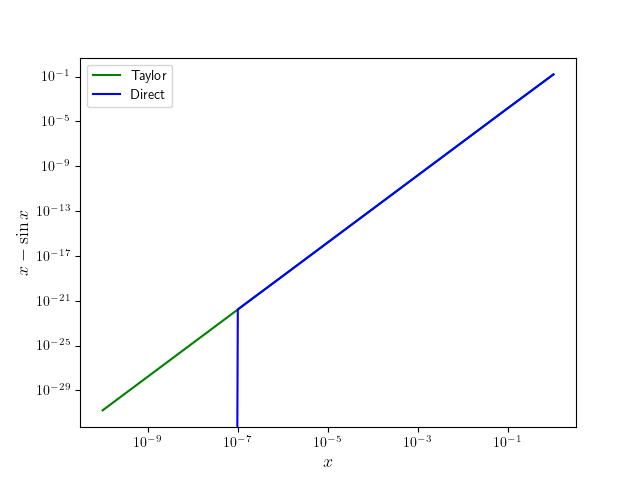
\includegraphics[width=0.8\textwidth]{Second_Week_1.png}
    \caption{直接计算与用泰勒展开计算结果}
    \label{pic 3}
\end{figure}
\\\indent可以看到两种方法的计算结果在$10^{-7}$量级以上极其相近,这也就说明了泰勒展开的近似较为准确。但直接计算的方法在
$10^{-7}$量级以下发生严重偏移,这正是相减相消后精度不够导致的。\\
\indent并且我们知道$x-\sin{x} \sim x^{3}(x\rightarrow0)$,这也和图\ref{pic 3}中图像的线性以及直线的斜率相符合。

\subsection{对\ref{2}的解答}
易见$y_{0}=e-1$,故计算$y_{0}$时会发生舍入误差,若按照递推公式直接迭代计算$y_{n}$,这个舍入误差
和每次迭代时计算$e$的舍入误差因多次与远大于一的数相乘而变得十分巨大,导致算法不稳定。
\indent通过分部积分,我们可以得到$y_{n}$的递推公式:
\begin{equation}
    y_{n+1}=e-(n+1)y_{n}\notag
\end{equation}
利用上述递推公式我们可以理论上地算出:
\begin{equation}
    \int_{0}^{1} x^{n}e^{x} dx = (-1)^n n! (e-1) + (-1)^n n! e \sum_{k=1}^{n} (-1)^k \frac{1}{k!} \notag
\end{equation}
\\注意到
\begin{equation}
    e^{-x}-1=\sum_{k=1}^{\infty}\frac{(-x)^k}{k!}=\sum_{k=1}^{n}\frac{(-x)^k}{k!} + R_{n}(x)\notag
\end{equation}
其中,$R_n(x) = \frac{e^{-cx} }{(n+1)!}x^{n+1},c\in(0,1)$。\\
故有
\begin{equation}
    \left|\int_{0}^{1} x^{n}e^{x} dx \right|= \left|(-1)^n n! (e-1) + (-1)^n n! e (e^{-1}-1-R_{n}(1))\right|
    = \frac{e^{1-c}}{(n+1)}
    \leq \frac{e}{n+1}\notag
\end{equation}
故当$n$足够大时(这里我们取界限为$2^{24}$),我们可以认为$y_{n}=0$,并将递推公式改写为:
\begin{equation}
    y_{n}=\frac{e-y_{n+1}}{n+1}\notag
\end{equation}
如此由后向前逆向递推,可以使误差不断乘远小于1的数从而阶乘级缩小。\\
\indent考虑到$y_{n}$十分接近$0$,计算的近似值可能会在$0$的上下波动,我们对两种方法计算出的$\left|y_{i}\right|,i=1,2,\cdots,100$进行作图:
\begin{figure}[h]
    \centering
    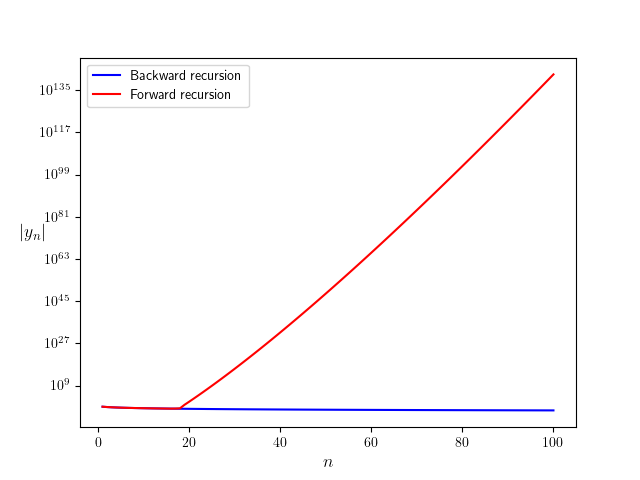
\includegraphics[width=0.8\textwidth]{Second_Week_2.png}
    \caption{两种递推法算出的$y_{n}$}
    \label{pic 4}
\end{figure}
\\\indent可以看到正向递推法求得的$y_{n}$在$n$不较小的情况下表现出了指数级增长,这显然不符合$y_{n}$的单调变化。
而逆向递推法求得的$y_{n}$始终平稳地减小,这是符合实际的。

\subsection{对\ref{3}的解答}
使用递推公式及初值可以求得$x_{n}=\frac{1}{3^{n}}$。使用python程序直接计算即可,但要注意的是应计算$\frac{1}{3^{n}}$
而非$\left(\frac{1}{3}\right)^{n}$,后者会将舍入误差幂次计算,从而增大误差(见附录代码中的)
我们使用python程序,将数字都进行单精度表示后
利用递推公式迭代计算$x_{n}(n\geq2)$,并计算其与单精度表示的$\frac{1}{3^{n}}$之差,得到下图:
\begin{figure}[h]
    \centering
    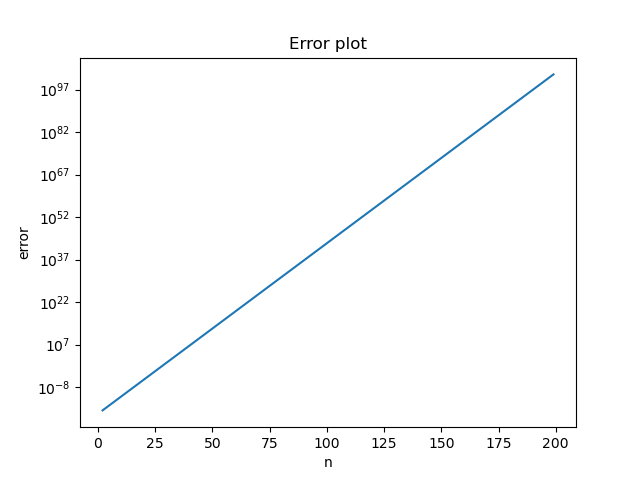
\includegraphics[width=0.8\textwidth]{Second_Week_3A.png}
    \caption{$x_{n}$与$\frac{1}{3^{n}}$之间的误差}
    \label{pic 1}
\end{figure}
\\\indent可以看到随着n的增大,误差呈指数型增长,在$n=200$是更是达到了惊人的$10^{97}$量级,说明递推地正向计算是不稳定的。
我们可以发现,误差主要来自于非$3$倍数的整数除以$3$发生的舍入误差在数列的正向递推中不断累积
($\frac{1}{3^{n}}$计算时也发生了舍入误差,但与数列递推产生的误差相比可以忽略不计),我们记
\begin{equation}
    x_{n}=\frac{1}{3^{n}}(1+\varepsilon_{n}) \label{(*)}
\end{equation}
记计算$\frac{1}{3}$时产生的舍入误差为$\varepsilon$。易见$\varepsilon_{0}=0$,$\varepsilon_{1}=\varepsilon$。
将(\ref{(*)})式代入递推公式得(事实上递推公式中计算$\frac{13}{3}$与$\frac{4}{3}$也会发生舍入误差,但当$n$不过小时,
此舍入误差的量级远远小于$\varepsilon_{n}$,故在下面的推导中忽略不计):
\begin{equation}
    \varepsilon^{n+1}=13\varepsilon_{n}-12\varepsilon_{n-1}(n\geq1)\notag
\end{equation}
解得$\varepsilon_{n}=\frac{1}{11}(12^{n}-1)\varepsilon$,故可见实际误差(即$x_{n}$与$\frac{1}{3^{n}}$之间的误差)满足:
\begin{equation}
    \widehat{\varepsilon_{n}}=\frac{1}{11}\left[4^{n}-\left(\frac{1}{3}\right)^{n}\right]\varepsilon\approx\frac{4^{n}}{11}\varepsilon\notag
\end{equation}
$\widehat{\varepsilon_{n}}$确实如图\ref{pic 1}关于$n$指数增长。
并且结合Week 1的上机作业可知,$\varepsilon_{mach} \approx 5.96046 \times 10^{-8}$,
$\frac{1}{3}$的舍入误差$\varepsilon$量级上应比$\varepsilon_{mach}$小,
于是$\varepsilon_{2}\approx\frac{16}{11}\varepsilon$的量级小于$10^{-8}$,与图\ref{pic 1}的起始点位置相符合。\\
\\我们令$x_{0}=1$,$x_{1}=4$,得到误差图如下:
\begin{figure}[h]
    \centering
    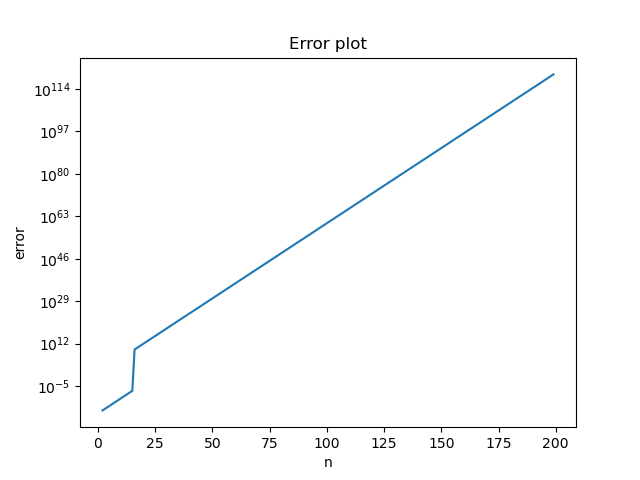
\includegraphics[width=0.8\textwidth]{Second_Week_3B.png}
    \caption{$x_{n}$与$\frac{1}{3^{n}}$之间的误差}
    \label{pic 2}
\end{figure}
\\可以看到误差也是呈指数型增长。事实上,若类似上文的定义,应有$\varepsilon_{0}=\varepsilon_{1}=0$,那为何还会发生舍入误差的累积呢?
这是因为其实由于计算$\frac{13}{3}$与$\frac{4}{3}$时发生的舍入误差,$\varepsilon_{2}\neq0$,故同前推导,误差依然会呈指数增长。
但此处与上例不同的是,折线在$n=15$处发生了一次“突变”,我认为这是$\varepsilon_{i}(i=2,3\cdots,15)$
不足以远大于计算$\frac{13}{3}$与$\frac{4}{3}$时发生的舍入误差导致的。


\section{结果分析}



\section{附录:程序代码}
\begin{lstlisting}

\end{lstlisting}
\end{document}
